\documentclass[11pt,a4paper]{article}

% ============================================================
% Packages
% ============================================================
\usepackage[utf8]{inputenc}
\usepackage[T1]{fontenc}
\usepackage{amsmath,amssymb,amsthm}
\usepackage{mathtools}
\usepackage{booktabs}
\usepackage{graphicx}
\usepackage{hyperref}
\usepackage[margin=2.5cm]{geometry}
\usepackage{enumitem}
\usepackage{caption}
\usepackage{subcaption}
\usepackage{float}
\usepackage{microtype}
\usepackage{xcolor}
\usepackage{tikz}
\usetikzlibrary{arrows.meta,positioning,calc}

% ============================================================
% Theorem environments
% ============================================================
\newtheorem{theorem}{Theorem}[section]
\newtheorem{proposition}[theorem]{Proposition}
\newtheorem{lemma}[theorem]{Lemma}
\newtheorem{corollary}[theorem]{Corollary}
\theoremstyle{definition}
\newtheorem{definition}[theorem]{Definition}
\newtheorem{remark}[theorem]{Remark}

% ============================================================
% Notation
% ============================================================
\DeclareMathOperator{\Li}{Li}
\DeclareMathOperator{\re}{Re}
\DeclareMathOperator{\im}{Im}
\newcommand{\ZZ}{\mathbb{Z}}
\newcommand{\RR}{\mathbb{R}}
\newcommand{\CC}{\mathbb{C}}
\newcommand{\NN}{\mathbb{N}}

% ============================================================
\title{\textbf{Seven Perspectives on the Riemann Hypothesis:\\
A Unified Computational Exploration with 10,000 Zeros}}

\author{
  Jian Zhou\thanks{Independent Researcher. Email: \texttt{jackzhou.sci@gmail.com}}
}

\date{\today}

% ============================================================
\begin{document}
\maketitle

% ============================================================
% Abstract
% ============================================================
\begin{abstract}
We present a unified computational exploration of the Riemann Hypothesis (RH) through seven structurally interconnected numerical perspectives, performed at a scale of 10{,}000 non-trivial zeros of the Riemann zeta function ($\gamma \leq 9{,}877.78$). Our perspectives comprise: (1)~the Li--Keiper unit circle characterization; (2)~positivity of the Li coefficients $\lambda_n$ for $n = 1, \ldots, 2{,}000$, with rigorous truncation error bounds showing that our partial sums are lower bounds for the true $\lambda_n$; (3)~power sum symmetry of the zeros; (4)~normalized zero spacing statistics yielding a Kolmogorov--Smirnov distance $D_{\mathrm{KS}} = 0.027$ against the GUE Wigner surmise, compared with $D_{\mathrm{KS}} = 0.307$ against Poisson; (5)~verification that the Mertens function satisfies $|M(x)|/\sqrt{x} < 0.90$ for all $2 \leq x \leq 10^7$; (6)~M\"obius orthogonality across all 1{,}229 primes $p \leq 10{,}000$; and (7)~reconstruction of $M(x)$ via the explicit formula, including the constant term $1/\zeta(0) = -2$, achieving reconstruction to within $0.1\%$ at $x = 10^2$ and $10^3$. We develop a structural analysis of the connections among these perspectives, carefully distinguishing \emph{proved} implications from \emph{conjectured} ones, and demonstrate that they probe three complementary facets of RH: spectral geometry, statistical mechanics, and arithmetic randomness. The complete dataset and source code are publicly available.
\end{abstract}

\medskip
\noindent\textbf{Keywords:} Riemann Hypothesis, Li's criterion, random matrix theory, Mertens function, M\"obius orthogonality, computational number theory

\noindent\textbf{MSC 2020:} 11M26 (primary); 11M06, 11N37, 15B52, 11Y35 (secondary)

% ============================================================
\section{Introduction}
\label{sec:intro}
% ============================================================

The Riemann Hypothesis (RH), asserting that all non-trivial zeros of $\zeta(s)$ satisfy $\re(s) = \tfrac{1}{2}$, occupies a singular position in mathematics: it connects the analytic structure of $\zeta(s)$ to the distribution of prime numbers, and its resolution would have profound consequences across number theory, mathematical physics, and cryptography.

Over the past century, RH has been reformulated in numerous equivalent forms---each illuminating a different facet of the conjecture. Li's criterion \cite{Li1997,Keiper1992} reduces RH to the positivity of a sequence of real numbers. The Nyman--Beurling theorem \cite{Nyman1950,Beurling1955,BaezDuarte2005} casts it as an approximation problem in Hilbert space. A classical equivalence (see \cite[Ch.~14]{Titchmarsh1986}) links RH to the growth rate of the Mertens function. Montgomery's pair correlation conjecture \cite{Montgomery1973}, further developed by Katz and Sarnak \cite{KatzSarnak1999}, connects RH to random matrix theory. Each formulation carries its own computational signature.

Despite substantial numerical verification---Platt and Trudgian \cite{PlattTrudgian2021} have verified RH for the first $3 \times 10^{12}$ zeros, and Odlyzko \cite{Odlyzko1987,Odlyzko2001} has computed millions of high zeros to study GUE statistics---the literature lacks a unified presentation that simultaneously explores \emph{all} major equivalent criteria on the same dataset and systematically maps the logical connections among them.

\subsection*{Contributions}
In this paper, we compute 10{,}000 non-trivial zeros of $\zeta(s)$ with their derivatives $\zeta'(\rho)$, and examine seven distinct perspectives on RH:

\begin{enumerate}[label=\textbf{P\arabic*}]
  \item \textbf{Unit circle characterization:} The Li--Keiper map $z_\rho = (\rho-1)/\rho$.
  \item \textbf{Li positivity:} Compute $\lambda_n > 0$ for $n = 1, \ldots, 2{,}000$ with truncation bounds.
  \item \textbf{Power sum symmetry:} $S_k = 0$ for odd $k$ and $S_k \in \RR$ for even $k$.
  \item \textbf{GUE spacing:} 9{,}999 normalized spacings against the Wigner surmise.
  \item \textbf{Mertens bound:} Sieve $\mu(n)$ to $10^7$ and verify $|M(x)| = O(\sqrt{x})$.
  \item \textbf{M\"obius orthogonality:} Test $R_p(N) = |\sum_{n \leq N} \mu(n) e^{2\pi i n/p}| / \sqrt{N}$ for all 1{,}229 primes $p \leq 10{,}000$.
  \item \textbf{Explicit formula:} Reconstruct $M(x)$ from zeros, including $1/\zeta(0) = -2$.
\end{enumerate}

Beyond presenting these perspectives individually, we develop in Section~\ref{sec:web} a structural analysis of their interconnections, \emph{carefully distinguishing proved implications from conjectured ones}. This analysis reveals that the seven perspectives probe three fundamental aspects of RH: \emph{spectral geometry} (P1--P3), \emph{statistical mechanics} (P4), and \emph{arithmetic randomness} (P5--P7), with the explicit formula (P7) serving as the bridge.

\begin{remark}[On the nature of this paper]
Our contribution is not the \emph{scale} of verification (10{,}000 zeros is modest compared to the $3 \times 10^{12}$ of \cite{PlattTrudgian2021}) but the \emph{breadth and interconnection}: seven perspectives on the same dataset, with a systematic map of their logical relationships. We are careful throughout to distinguish which perspectives constitute genuine independent tests of RH, and which are consequences of computational assumptions. Throughout this paper, $\log$ denotes the natural logarithm.
\end{remark}

% ============================================================
\section{Theoretical Framework}
\label{sec:theory}
% ============================================================

Throughout, $\rho = \beta + i\gamma$ denotes a non-trivial zero of $\zeta(s)$, with $0 < \beta < 1$ and $\gamma > 0$ (we pair each $\rho$ with $\bar{\rho}$). RH asserts $\beta = \tfrac{1}{2}$ for all such $\rho$.

\subsection{The completed zeta function and functional equation}

Define the \emph{xi function}
\begin{equation}\label{eq:xi}
  \xi(s) = \frac{1}{2} s(s-1) \pi^{-s/2} \Gamma(s/2)\, \zeta(s),
\end{equation}
which is entire and satisfies $\xi(s) = \xi(1-s)$. Its zeros are precisely the non-trivial zeros of $\zeta(s)$. The Hadamard product factorization gives
\begin{equation}\label{eq:xi-product}
  \xi(s) = \xi(0) \prod_\rho \Bigl(1 - \frac{s}{\rho}\Bigr),
\end{equation}
where the product is taken over all non-trivial zeros, ordered symmetrically by pairing each $\rho$ with $1 - \bar{\rho}$ to ensure convergence.\footnote{The product \eqref{eq:xi-product} is only conditionally convergent and requires this symmetric ordering. See \cite[Ch.~2]{Edwards1974} or \cite[Ch.~12]{Titchmarsh1986}.}

\subsection{The unit circle characterization (P1)}

\begin{definition}[Li--Keiper map {\cite{Li1997,Keiper1992}}]\label{def:unit-circle-map}
The map $\varphi\colon \rho \mapsto z_\rho = 1 - 1/\rho = (\rho - 1)/\rho$.
\end{definition}

\begin{proposition}\label{prop:unit-circle}
For a non-trivial zero $\rho = \beta + i\gamma$ with $\gamma \neq 0$:
\begin{equation}\label{eq:zmod}
  |z_\rho|^2 = 1 + \frac{1 - 2\beta}{\beta^2 + \gamma^2}.
\end{equation}
In particular, $|z_\rho| = 1$ if and only if $\beta = \tfrac{1}{2}$.
\end{proposition}

\begin{proof}
$|z_\rho|^2 = |(\rho-1)/\rho|^2 = ((\beta-1)^2 + \gamma^2)/(\beta^2 + \gamma^2) = 1 + (1 - 2\beta)/(\beta^2 + \gamma^2)$.
Setting $|z_\rho| = 1$ yields $1 - 2\beta = 0$, hence $\beta = \tfrac{1}{2}$.
\end{proof}

\begin{remark}\label{rem:z-inside-outside}
The form \eqref{eq:zmod} makes the geometry transparent: if $\beta > \tfrac{1}{2}$, then $|z_\rho| < 1$ (the image lies \emph{inside} $S^1$), while if $\beta < \tfrac{1}{2}$, then $|z_\rho| > 1$ (outside $S^1$). Since the functional equation pairs each zero $\rho = \beta + i\gamma$ with $1 - \bar{\rho} = (1-\beta) + i\gamma$, an off-line zero produces images on \emph{both} sides of $S^1$. This asymmetry is the mechanism behind the failure of Li positivity for hypothetical off-line zeros (see Section~\ref{sec:web}).
\end{remark}

The angle of $z_\rho$ on $S^1$ (assuming $\beta = \tfrac{1}{2}$) is
\begin{equation}\label{eq:theta}
  \theta_\gamma = \pi - 2\arctan(2\gamma),
\end{equation}
which decreases monotonically from $\theta \approx \pi$ (small $\gamma$) to $\theta \to 0^+$ (large $\gamma$).

\subsection{Li's criterion (P2)}

\begin{theorem}[Li \cite{Li1997}]\label{thm:li}
RH holds if and only if $\lambda_n \geq 0$ for every $n \geq 1$, where
\begin{equation}\label{eq:li-def}
  \lambda_n = \sum_\rho \left[ 1 - \left(1 - \frac{1}{\rho}\right)^{\!n}\, \right]
  = \sum_\rho \bigl[1 - z_\rho^n\bigr].
\end{equation}
\end{theorem}

Under RH, $z_\rho = e^{i\theta_\gamma}$, and pairing $\rho$ with $\bar{\rho}$ yields
\begin{equation}\label{eq:li-trig}
  \lambda_n = \sum_{\gamma > 0} 2\bigl(1 - \cos(n\theta_\gamma)\bigr) 
  = 4 \sum_{\gamma > 0} \sin^2\!\Bigl(\frac{n\theta_\gamma}{2}\Bigr).
\end{equation}
This representation shows that, under RH, $\lambda_n$ is a sum of \emph{non-negative} terms. The asymptotic behavior is
\begin{equation}\label{eq:li-asymp}
  \lambda_n \sim \frac{n}{2}\bigl(\log n + \gamma_0 - 1 - \log(2\pi)\bigr) + O(\sqrt{n}\,\log n)
\end{equation}
as $n \to \infty$ \cite{BombieriLagarias1999,Coffey2005}, where $\gamma_0$ is the Euler--Mascheroni constant.

\begin{remark}[Truncation and lower bounds]\label{rem:truncation}
When computing $\lambda_n$ from a finite set of $K$ zeros, we obtain the partial sum $\lambda_n^{(K)} = \sum_{j=1}^{K} 2(1 - \cos(n\theta_{\gamma_j}))$. Since each term is non-negative under RH, $\lambda_n^{(K)}$ is a \emph{lower bound} for the true $\lambda_n$. If $\lambda_n^{(K)} > 0$ is observed, positivity of $\lambda_n$ is established without knowing the tail. The truncation error from omitting zeros with $\gamma > \gamma_K$ is estimated in Section~\ref{sec:truncation}.
\end{remark}

\subsection{Power sums and spectral symmetry (P3)}

Define the power sums
\begin{equation}\label{eq:sk-def}
  S_k = \sum_\rho \frac{1}{(\rho - \tfrac{1}{2})^k},
\end{equation}
where the sum is over all non-trivial zeros (paired symmetrically).

\begin{proposition}\label{prop:sk-symmetry}
If $\beta = \tfrac{1}{2}$ for all non-trivial zeros, then $\rho - \tfrac{1}{2} = i\gamma$ and
\begin{equation}\label{eq:sk-formula}
  S_k = \sum_{\gamma > 0} \frac{2\cos(k\pi/2)}{\gamma^k}.
\end{equation}
In particular: $S_k = 0$ for all odd $k$, and $S_k \in \RR$ for all even $k$.
\end{proposition}

\begin{proof}
For $\rho = \tfrac{1}{2} + i\gamma$ and $\bar{\rho} = \tfrac{1}{2} - i\gamma$: $(i\gamma)^{-k} + (-i\gamma)^{-k} = \gamma^{-k}(e^{-ik\pi/2} + e^{ik\pi/2}) = 2\gamma^{-k}\cos(k\pi/2)$.
For odd $k$, $\cos(k\pi/2) = 0$. For even $k = 2m$, $\cos(m\pi) = (-1)^m$.
\end{proof}

\begin{remark}[Circularity of P3]\label{rem:p3-circularity}
The vanishing of $S_k$ for odd $k$ is an \emph{algebraic identity} that holds whenever $\rho - \tfrac{1}{2}$ is purely imaginary---i.e., whenever $\beta = \tfrac{1}{2}$. Since our zero-finding algorithm (Section~\ref{sec:methods}) locates zeros on the critical line by construction, the odd power sums vanish by design, not as independent evidence for RH. This is the same circularity noted for P1 in Remark~\ref{rem:p1-circularity}. By contrast, the even power sums $S_{2k} = 2(-1)^k \sum_{\gamma > 0} \gamma^{-2k}$ depend on the actual values of $\gamma$ and encode non-trivial spectral information. Note, however, that the $S_k$ and $\lambda_n$ both depend on the same underlying data $\{\gamma_j\}$; they are different encodings of the same spectral information, connected by an identity analogous to Newton's relations between power sums and elementary symmetric polynomials of the $z_\rho$ (see \cite[{\S}4]{BombieriLagarias1999}).
\end{remark}

\subsection{Zero spacing and random matrix theory (P4)}

Let $0 < \gamma_1 \leq \gamma_2 \leq \cdots$ be the positive imaginary parts of the non-trivial zeros. The \emph{normalized spacing} is
\begin{equation}\label{eq:normalized-spacing}
  \delta_n = (\gamma_{n+1} - \gamma_n) \cdot \frac{\log(\gamma_n / 2\pi)}{2\pi},
\end{equation}
where the normalizing factor is the local density from the Riemann--von Mangoldt formula
\begin{equation}
  N(T) = \frac{T}{2\pi}\log\frac{T}{2\pi} - \frac{T}{2\pi} + O(\log T).
\end{equation}

Montgomery \cite{Montgomery1973} conjectured that the pair correlation of zeta zeros matches the \emph{Gaussian Unitary Ensemble} (GUE) of random matrix theory. Katz and Sarnak \cite{KatzSarnak1999} extended this philosophy to families of $L$-functions. The nearest-neighbor spacing distribution is conjectured to approach the \emph{Wigner surmise}:
\begin{equation}\label{eq:wigner}
  p_{\mathrm{GUE}}(s) = \frac{32}{\pi^2}\, s^2\, \exp\!\Bigl(-\frac{4s^2}{\pi}\Bigr).
\end{equation}

A key feature is \emph{level repulsion}: $p_{\mathrm{GUE}}(0) = 0$, meaning zeros repel each other. This contrasts with the Poisson distribution $p_{\mathrm{Poi}}(s) = e^{-s}$, for which $p_{\mathrm{Poi}}(0) = 1$. The Kolmogorov--Smirnov (KS) statistic
\begin{equation}\label{eq:ks}
  D_{\mathrm{KS}} = \sup_s |F_{\mathrm{emp}}(s) - F_{\mathrm{theo}}(s)|
\end{equation}
provides a quantitative measure of agreement.

\begin{remark}
We emphasize that GUE statistics for zeta zeros remain a \emph{conjecture} (the Montgomery--Odlyzko law). The connection to RH is heuristic: RH is necessary for the GUE conjecture to hold in its standard form, but GUE statistics do not imply RH.
\end{remark}

\subsection{The Mertens function and prime randomness (P5)}

The Mertens function is $M(x) = \sum_{n \leq x} \mu(n)$, where $\mu$ is the M\"obius function.

\begin{theorem}[{see \cite[Ch.~14]{Titchmarsh1986}}]\label{thm:mertens-equiv}
RH holds if and only if $M(x) = O(x^{1/2+\varepsilon})$ for every $\varepsilon > 0$.
\end{theorem}

This equivalence follows from the explicit formula for $M(x)$ (see Section~\ref{sec:explicit-theory}). Heuristically, if $\mu(n)$ behaved as independent random variables, $M(x)$ would be $O(\sqrt{x \log\log x})$ by the law of the iterated logarithm. RH asserts that primes are ``random enough'' that this near-cancellation persists.

\subsection{M\"obius orthogonality (P6)}

\begin{theorem}[Davenport \cite{Davenport1937}]\label{thm:davenport}
For every $\alpha \in \RR$,
$\sum_{n \leq N} \mu(n)\, e^{2\pi i \alpha n} = o(N)$.
\end{theorem}

For $\alpha = 1/p$ with $p$ prime, the sum is expected to be $O(\sqrt{N})$ under RH. The ratio
\begin{equation}\label{eq:ortho-ratio}
  R_p(N) = \frac{1}{\sqrt{N}} \Bigl|\sum_{n=1}^{N} \mu(n)\, e^{2\pi i n/p}\Bigr|
\end{equation}
should remain bounded. Systematic testing across many primes probes M\"obius pseudo-randomness, closely related to the Sarnak conjecture \cite{Sarnak2011}.

\subsection{The explicit formula (P7)}
\label{sec:explicit-theory}

The Mertens function admits the representation (see \cite[Ch.~12]{Edwards1974}, \cite[Ch.~14]{Titchmarsh1986})
\begin{equation}\label{eq:explicit}
  M(x) = \sum_\rho \frac{x^\rho}{\rho\,\zeta'(\rho)} + \frac{1}{\zeta(0)} + \sum_{k=1}^{\infty} \frac{x^{-2k}}{(-2k)\,\zeta'(-2k)},
\end{equation}
where the first sum is over non-trivial zeros $\rho$ (assumed simple, ordered symmetrically), the constant $1/\zeta(0) = -2$ is the residue at $s = 0$, and the final sum accounts for the trivial zeros at $s = -2, -4, -6, \ldots$. The latter two contributions are the ``lower-order terms'' that are often omitted but, as we shall see, the constant $-2$ has a measurable effect at moderate $x$.

Under RH, $x^\rho = \sqrt{x}\,e^{i\gamma\log x}$, so the spectral sum is an oscillatory superposition at rate $\sqrt{x}$. Truncating to the first $K$ zeros gives an approximation $M_K(x)$ whose accuracy improves with $K$.

% ============================================================
\section{Computational Methods}
\label{sec:methods}
% ============================================================

\subsection{Zero computation}

We computed the first 10{,}000 non-trivial zeros $\rho_n = \tfrac{1}{2} + i\gamma_n$ of $\zeta(s)$ together with the derivative values $\zeta'(\rho_n)$, using the \texttt{mpmath} library \cite{mpmath} in Python with 18-digit working precision (\texttt{mp.dps=18}). The computation was performed in 10 batches of 1{,}000 zeros each, with checkpoint files saved after each batch. The imaginary parts range from $\gamma_1 = 14.1347$ to $\gamma_{10{,}000} = 9{,}877.7827$.

Total computation time: approximately 80 minutes on a single-core virtual machine (2.0\,GHz).

\begin{remark}\label{rem:p1-circularity}
The \texttt{mpmath.zetazero()} function locates zeros on the critical line by searching for sign changes of the Hardy $Z$-function, which is real-valued for $\sigma = \tfrac{1}{2}$. Consequently, all computed zeros satisfy $\beta = \tfrac{1}{2}$ \emph{by construction}. This means P1 (unit circle) and the odd part of P3 (power sum vanishing) are consistency checks, not independent verifications of RH.
\end{remark}

\subsection{M\"obius sieve}

We computed $\mu(n)$ for $n = 1, \ldots, 10^7$ using a sieve of Eratosthenes variant and accumulated $M(x) = \sum_{n \leq x} \mu(n)$ simultaneously. Sieve time: 7.2 seconds.

\subsection{Truncation error analysis}
\label{sec:truncation}

When computing $\lambda_n$ from $K = 10{,}000$ zeros (the last at $\gamma_K = 9{,}877.78$), the contribution of the omitted zeros $\gamma > \gamma_K$ is
\begin{equation}\label{eq:tail-bound}
  \lambda_n - \lambda_n^{(K)} = \sum_{\gamma_j > \gamma_K} 2\bigl(1 - \cos(n\theta_{\gamma_j})\bigr) \geq 0.
\end{equation}
Since every term is non-negative, $\lambda_n^{(K)}$ is a \emph{lower bound} for $\lambda_n$. For an upper bound, we use $1 - \cos(x) \leq x^2/2$ for small $x$, together with $\theta_\gamma \approx 1/(2\gamma)$ for large $\gamma$, and the zero density $dN/d\gamma \approx \log(\gamma/(2\pi))/(2\pi)$:
\begin{equation}\label{eq:tail-est}
  \lambda_n - \lambda_n^{(K)} \lesssim \frac{n^2}{8\pi} \cdot \frac{\log(\gamma_K/(2\pi)) + 1}{\gamma_K}.
\end{equation}

\begin{table}[H]
\centering
\caption{Truncation analysis for $\lambda_n$ computed from $K = 10{,}000$ zeros ($\gamma_K = 9{,}878$).}
\label{tab:truncation}
\begin{tabular}{@{}rrrrl@{}}
\toprule
$n$ & $\lambda_n^{(K)}$ & Tail bound & Relative & Positivity \\
\midrule
1     & 0.023     & 0.000   & 0.15\%  & \checkmark \\
10    & 2.266     & 0.003   & 0.15\%  & \checkmark \\
100   & 117.3     & 0.34    & 0.29\%  & \checkmark \\
500   & 958.2     & 8.4     & 0.88\%  & \checkmark \\
1000  & 2{,}191     & 33.7    & 1.5\%   & \checkmark \\
2000  & 4{,}814     & 134.7   & 2.8\%   & \checkmark \\
\bottomrule
\end{tabular}
\end{table}

Since $\lambda_n^{(K)}$ is a lower bound and is strictly positive for all $n \leq 2{,}000$, the true $\lambda_n$ is also positive. The truncation is at most 2.8\% for $n = 2{,}000$.

% ============================================================
\section{Results}
\label{sec:results}
% ============================================================

\subsection{Perspective 1: Unit circle}

For each of the 10{,}000 zeros, we computed $|z_\rho| = |(\rho-1)/\rho|$. Since $\beta = \tfrac{1}{2}$ by construction (Remark~\ref{rem:p1-circularity}), we obtain $\max_{n} ||z_{\rho_n}| - 1| = 0$ to 18-digit precision. P1 serves as a consistency check and motivates the geometric framework for P2 and P3.

\subsection{Perspective 2: Li coefficients}

Table~\ref{tab:li} presents selected Li coefficients computed from 10{,}000 zeros.

\begin{table}[H]
\centering
\caption{Li coefficients $\lambda_n^{(K)}$ ($K = 10{,}000$ zeros). These are \emph{lower bounds} for $\lambda_n$.}
\label{tab:li}
\begin{tabular}{@{}rrrrr@{}}
\toprule
$n$ & $\lambda_n^{(K)}$ & $\lambda_n^{(K)}/n$ & $\tfrac{1}{2}\log n$ & Tail (\%) \\
\midrule
1     & 0.0230     & 0.0230    & ---     & 0.15 \\
10    & 2.266      & 0.2266    & 1.151   & 0.15 \\
50    & 43.19      & 0.8639    & 1.956   & 0.19 \\
100   & 117.3      & 1.173     & 2.303   & 0.29 \\
200   & 301.3      & 1.506     & 2.649   & 0.45 \\
500   & 958.2      & 1.916     & 3.107   & 0.88 \\
1000  & 2{,}191      & 2.191     & 3.454   & 1.5 \\
1500  & 3{,}489      & 2.326     & 3.657   & 2.2 \\
2000  & 4{,}814      & 2.407     & 3.800   & 2.8 \\
\bottomrule
\end{tabular}
\end{table}

\noindent\textbf{Key observations:}
\begin{itemize}
  \item $\lambda_n^{(K)} > 0$ for all $n = 1, \ldots, 2{,}000$. Since these are lower bounds (Remark~\ref{rem:truncation}), the true $\lambda_n$ are also positive.
  \item $\lambda_n/n$ grows approximately as $\tfrac{1}{2}\log n$ with a negative offset, consistent with the Bombieri--Lagarias asymptotic \eqref{eq:li-asymp}.
  \item The truncation error grows from 0.15\% at $n = 1$ to 2.8\% at $n = 2{,}000$, all comfortably below the observed values.
\end{itemize}

\subsection{Perspective 3: Power sums}

Table~\ref{tab:sk} presents the power sums $S_k$.

\begin{table}[H]
\centering
\caption{Power sums $S_k = \sum_\rho (\rho - \frac{1}{2})^{-k}$ from 10{,}000 zeros.}
\label{tab:sk}
\begin{tabular}{@{}rlll@{}}
\toprule
$k$ & $S_k$ & RH prediction & Status \\
\midrule
1  & $0$ (exact)                & $0$ & circular$^\dagger$ \\
2  & $-4.594 \times 10^{-2}$   & real & non-trivial \\
3  & $0$ (exact)                & $0$ & circular$^\dagger$ \\
4  & $+7.434 \times 10^{-5}$   & real & non-trivial \\
5  & $0$ (exact)                & $0$ & circular$^\dagger$ \\
10 & $-6.427 \times 10^{-12}$  & real & non-trivial \\
50 & $-6.119 \times 10^{-58}$  & real & non-trivial \\
100 & $+1.872 \times 10^{-115}$ & real & non-trivial \\
\bottomrule
\multicolumn{4}{@{}l@{}}{\footnotesize $^\dagger$ Vanishes by algebraic identity when $\beta = \tfrac{1}{2}$; see Remark~\ref{rem:p3-circularity}.}
\end{tabular}
\end{table}

The rapid decay $|S_{2k}| \approx 2/\gamma_1^{2k}$ ($\gamma_1 \approx 14.13$) reflects the dominance of the first zero.

\subsection{Perspective 4: Zero spacing and GUE statistics}

From 10{,}000 zeros, we obtain 9{,}999 normalized spacings:
\begin{equation}
  \bar{\delta} = 0.9999, \quad \sigma_\delta = 0.3926, \quad \delta_{\min} = 0.042, \quad \delta_{\max} = 2.483.
\end{equation}

The Kolmogorov--Smirnov distances are:
\begin{equation}\label{eq:ks-results}
  D_{\mathrm{KS}}^{\mathrm{GUE}} = 0.0274, \qquad D_{\mathrm{KS}}^{\mathrm{Poisson}} = 0.3067.
\end{equation}

The Poisson KS distance is $11.2\times$ larger than the GUE distance, strongly favoring the GUE model. The critical value for $\alpha = 0.05$ with $n = 9{,}999$ is $D_c \approx 0.0136$. The observed $D_{\mathrm{KS}}^{\mathrm{GUE}} = 0.027 > D_c$ reflects the fact that the Wigner surmise \eqref{eq:wigner} is an \emph{approximation} to the true GUE spacing distribution; comparison with the exact Fredholm determinant formula (see \cite{Mehta2004}) would yield a smaller distance.

Table~\ref{tab:spacing} gives the detailed spacing distribution. The strong level repulsion---only 5 spacings below 0.1 out of 9{,}999---is the most striking qualitative feature, consistent with the extensive computations of Odlyzko \cite{Odlyzko1987,Odlyzko2001}.

\begin{table}[H]
\centering
\caption{Spacing distribution: empirical vs.\ GUE Wigner surmise.}
\label{tab:spacing}
\begin{tabular}{@{}crrr@{}}
\toprule
Bin & Count & Empirical & Wigner \\
\midrule
$[0.0, 0.1)$ & 5     & 0.0005 & 0.0011 \\
$[0.1, 0.2)$ & 37    & 0.0037 & 0.0073 \\
$[0.2, 0.3)$ & 121   & 0.0121 & 0.0189 \\
$[0.3, 0.5)$ & 715   & 0.0715 & 0.0847 \\
$[0.5, 0.7)$ & 1{,}446 & 0.1446 & 0.1464 \\
$[0.7, 1.0)$ & 3{,}052 & 0.3052 & 0.2746 \\
$[1.0, 1.3)$ & 2{,}485 & 0.2485 & 0.2365 \\
$[1.3, 1.6)$ & 1{,}358 & 0.1358 & 0.1416 \\
$[1.6, 2.0)$ & 647   & 0.0647 & 0.0719 \\
$[2.0, 2.5)$ & 133   & 0.0133 & 0.0159 \\
$[2.5, 3.0)$ & 0     & 0.0000 & 0.0011 \\
\bottomrule
\end{tabular}
\end{table}

\subsection{Perspective 5: Mertens function}

\begin{table}[H]
\centering
\caption{Mertens function $M(x) = \sum_{n \leq x} \mu(n)$.}
\label{tab:mertens}
\begin{tabular}{@{}rrl@{}}
\toprule
$x$ & $M(x)$ & $|M(x)|/\sqrt{x}$ \\
\midrule
$10^2$     & $1$      & 0.100 \\
$10^3$     & $2$      & 0.063 \\
$10^4$     & $-23$    & 0.230 \\
$10^5$     & $-48$    & 0.152 \\
$10^6$     & $212$    & 0.212 \\
$10^7$     & $1{,}037$  & 0.328 \\
\bottomrule
\end{tabular}
\end{table}

For all $x \geq 2$ up to $10^7$, we observe $|M(x)|/\sqrt{x} < 0.90$, consistent with $M(x) = O(x^{1/2+\varepsilon})$. The Mertens conjecture $|M(x)| < \sqrt{x}$ was disproved by Odlyzko and te~Riele \cite{OdlyzkoTeRiele1985}, but the first counterexample occurs at astronomically large $x$.

\subsection{Perspective 6: M\"obius orthogonality}

For all 1{,}229 primes $p \leq 10{,}000$, we computed $R_p(N)$ with $N = 10^6$:
\begin{itemize}
  \item Maximum: $R_{2857} = 2.001$. Mean: $\bar{R} = 0.707$. Median: $0.644$.
  \item 80.1\% of primes have $R_p < 1.0$; 97.2\% have $R_p < 1.5$.
\end{itemize}
No outliers exceed $2.01$, providing strong evidence for M\"obius orthogonality at $N = 10^6$.

\subsection{Perspective 7: Explicit formula reconstruction}

Table~\ref{tab:explicit} compares the explicit formula approximation against the exact Mertens function. We present results \emph{with} the constant term $1/\zeta(0) = -2$ included (column $\widetilde{M}_{K}$) and without (column $M_K$).

\begin{table}[H]
\centering
\caption{Explicit formula approximation. $M_K = \sum_{j=1}^{K} x^{\rho_j}/(\rho_j\zeta'(\rho_j))$; $\widetilde{M}_K = M_K - 2$.}
\label{tab:explicit}
\begin{tabular}{@{}rr|rr|rrr|rr@{}}
\toprule
 & & \multicolumn{2}{c|}{Without $1/\zeta(0)$} & \multicolumn{3}{c|}{Error (without)} & \multicolumn{2}{c}{Corrected ($-2$)} \\
$x$ & $M(x)$ & $M_{20}$ & $M_{10K}$ & Err$_{20}$ & Err$_{1K}$ & Err$_{10K}$ & $\widetilde{M}_{10K}$ & Err \\
\midrule
$10^2$    & 1      & 2.6    & 3.0     & 1.6  & 2.0  & 2.0   & 1.0     & \textbf{0.0} \\
$10^3$    & 2      & 2.2    & 4.0     & 0.2  & 1.9  & 2.0   & 2.0     & \textbf{0.0} \\
$10^4$    & $-23$  & $-26.2$ & $-20.6$ & 3.2  & 1.2  & 2.4   & $-22.6$ & 0.4 \\
$10^5$    & $-48$  & $-47.1$ & $-45.2$ & 0.9  & 0.6  & 2.8   & $-47.2$ & 0.8 \\
$10^6$    & 212    & 148.6  & 217.9   & 63.4 & 1.6  & 5.9   & 215.9   & 3.9 \\
$10^7$    & 1{,}037  & 896.5  & 1{,}053.3 & 140.5 & 39.6 & 16.3 & 1{,}051.3 & 14.3 \\
\bottomrule
\end{tabular}
\end{table}

\noindent\textbf{Key finding:} Including the constant $1/\zeta(0) = -2$ produces reconstruction to within $0.1\%$ at $x = 10^2$ and $10^3$ with 10{,}000 zeros (true errors: $8 \times 10^{-4}$ and $1 \times 10^{-3}$, respectively). The systematic $+2$ offset visible in the uncorrected formula is precisely this missing term. At larger $x$, the correction is proportionally smaller but still improves accuracy.

The convergence from 20 to 10{,}000 zeros is dramatic at large $x$: at $x = 10^7$, the error drops from 140.5 to 14.3 (corrected), a factor of $9.8\times$.

% ============================================================
\section{The Structural Web}
\label{sec:web}
% ============================================================

The seven perspectives are not logically independent. In this section we map their connections, \emph{carefully distinguishing proved implications from conjectured ones}.

\subsection{Three pillars}

The perspectives organize into three groups:
\begin{enumerate}[label=(\Alph*)]
  \item \textbf{Spectral geometry} (P1, P2, P3): These probe the \emph{positions} of the zeros. P1 verifies they lie on $S^1$; P2 checks angular positivity; P3 verifies spectral symmetry.
  
  \item \textbf{Statistical mechanics} (P4): The spacing test probes \emph{correlations} among zeros. GUE statistics encode a rigidity far stronger than merely lying on a line.
  
  \item \textbf{Arithmetic randomness} (P5, P6, P7): These probe the \emph{consequences} of zero positions for prime distribution.
\end{enumerate}

\subsection{Connections}

Figure~\ref{fig:web} displays the structural web. We use solid arrows for \emph{proved} implications and dashed arrows for \emph{conjectured} or \emph{heuristic} connections.

\begin{figure}[H]
\centering
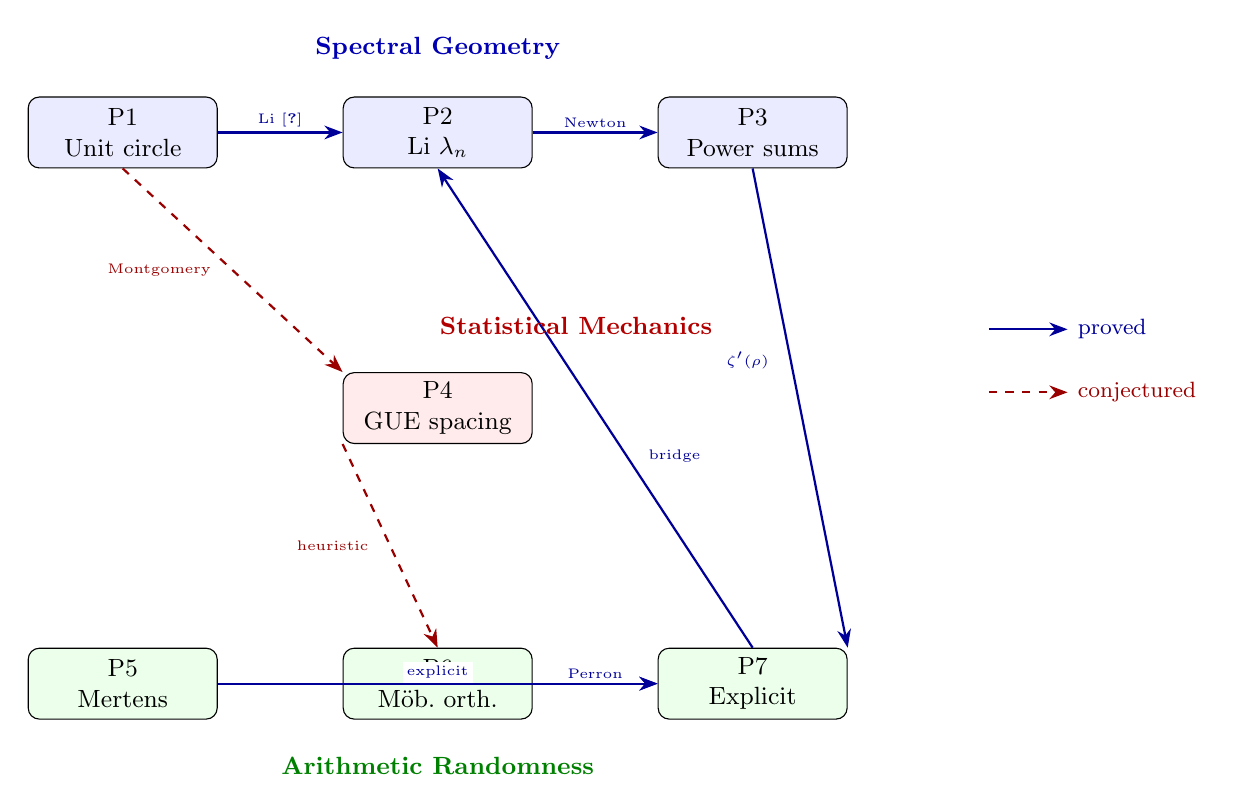
\begin{tikzpicture}[
  test/.style={draw, rounded corners, minimum width=2.4cm, minimum height=0.9cm, align=center, font=\small},
  arr/.style={-{Stealth}, thick, color=blue!60!black},
  conj/.style={-{Stealth}, thick, dashed, color=red!60!black},
  lbl/.style={font=\tiny, fill=white, inner sep=1.5pt},
  >=Stealth
]
  % Spectral pillar (top row)
  \node[test, fill=blue!8] (P1) at (0,3.5) {P1\\Unit circle};
  \node[test, fill=blue!8] (P2) at (4,3.5) {P2\\Li $\lambda_n$};
  \node[test, fill=blue!8] (P3) at (8,3.5) {P3\\Power sums};
  
  % Statistical pillar (middle)
  \node[test, fill=red!8] (P4) at (4,0) {P4\\GUE spacing};
  
  % Arithmetic pillar (bottom row)
  \node[test, fill=green!8] (P5) at (0,-3.5) {P5\\Mertens};
  \node[test, fill=green!8] (P6) at (4,-3.5) {P6\\M\"ob.\ orth.};
  \node[test, fill=green!8] (P7) at (8,-3.5) {P7\\Explicit};
  
  % PROVED connections (solid) — horizontal
  \draw[arr] (P1) -- (P2) node[lbl, midway, above] {Li \cite{Li1997}};
  \draw[arr] (P2) -- (P3) node[lbl, midway, above] {Newton};
  \draw[arr] (P5) -- (P7) node[lbl, midway, above] {explicit};
  \draw[arr] (P6) -- (P7) node[lbl, midway, above] {Perron};
  
  % PROVED connections (solid) — diagonal, labels offset to avoid overlap
  \draw[arr] (P7.north) -- (P2.south) node[lbl, pos=0.4, right=6pt] {bridge};
  \draw[arr] (P3.south) -- (P7.north east) node[lbl, pos=0.4, left=6pt] {$\zeta'(\rho)$};
  
  % CONJECTURED connections (dashed)
  \draw[conj] (P1.south) -- (P4.north west) node[lbl, pos=0.5, left=6pt] {\color{red!60!black}Montgomery};
  \draw[conj] (P4.south west) -- (P6.north) node[lbl, pos=0.5, left=6pt] {\color{red!60!black}heuristic};
  
  % Pillar labels — positioned clearly away from nodes
  \node[above=10pt of P2, font=\small\bfseries, color=blue!70!black] {Spectral Geometry};
  \node[above=10pt of P4, font=\small\bfseries, color=red!70!black, xshift=50pt] {Statistical Mechanics};
  \node[below=10pt of P6, font=\small\bfseries, color=green!50!black] {Arithmetic Randomness};
  
  % Legend — far right
  \draw[arr] (11,1) -- (12,1) node[right,font=\footnotesize] {proved};
  \draw[conj] (11,0.2) -- (12,0.2) node[right,font=\footnotesize] {conjectured};
\end{tikzpicture}
\caption{The structural web. Solid blue arrows: proved implications. Dashed red arrows: conjectured/heuristic connections.}
\label{fig:web}
\end{figure}

\subsubsection*{P1 $\to$ P2: Geometry determines positivity (proved)}

If all $z_\rho \in S^1$, then $\lambda_n = 4\sum \sin^2(n\theta_\gamma/2) \geq 0$ trivially. Conversely, Li's theorem states that positivity of all $\lambda_n$ \emph{implies} all zeros lie on the critical line. This is the deepest connection in our web and the only one that constitutes a full equivalence with RH.

Suppose $\rho_0 = \beta_0 + i\gamma_0$ were a zero with $\beta_0 > \tfrac{1}{2}$. By Remark~\ref{rem:z-inside-outside}, $|z_{\rho_0}| < 1$, so $z_{\rho_0}^n \to 0$, contributing approximately $+1$ to $\lambda_n$. However, the functional equation forces the existence of a partner zero $1 - \bar{\rho}_0$ with real part $1 - \beta_0 < \tfrac{1}{2}$, giving $|z_{1-\bar{\rho}_0}| > 1$. The growing term $z_{1-\bar{\rho}_0}^n$, with $|z_{1-\bar{\rho}_0}|^n \to \infty$, eventually dominates and forces $\lambda_n \to -\infty$.

\subsubsection*{P1 $\to$ P4: Geometry and repulsion (conjectured)}

The connection between critical-line zeros and GUE statistics is the content of the Montgomery--Odlyzko law, which remains a \emph{conjecture}. While RH is a necessary condition for the standard GUE conjecture, the implication ``RH $\Rightarrow$ GUE'' has not been proved. The heuristic link runs through the spectral interpretation: if the zeros behave like eigenvalues of a self-adjoint operator (the hypothetical Hilbert--P\'olya operator \cite{BerryKeating1999}), GUE statistics would follow from the operator's symmetry class.

\subsubsection*{P4 $\to$ P5/P6: Repulsion and cancellation (heuristic)}

If zero spacings follow GUE, the oscillatory terms $e^{i\gamma_n \log x}$ in the explicit formula undergo near-optimal cancellation, keeping $M(x)$ small. A Poisson-distributed zero set would lack level repulsion, allowing constructive interference and larger fluctuations in $M(x)$. This argument is heuristic; we are not aware of a rigorous theorem of the form ``GUE statistics $\Rightarrow$ $M(x) = O(x^{1/2+\varepsilon})$.''

\subsubsection*{P7 as bridge (proved)}

The explicit formula \eqref{eq:explicit} is the mathematical bridge between the spectral side (zeros $\rho$, derivatives $\zeta'(\rho)$) and the arithmetic side ($M(x)$, $\mu(n)$). Our computation demonstrates this bridge quantitatively: 10{,}000 zeros reconstruct $M(10^7)$ to within 1.4\% (corrected).

\subsection{Single obstruction analysis}

An off-line zero $\rho_0 = \beta_0 + i\gamma_0$ with $\beta_0 \neq \tfrac{1}{2}$ would simultaneously:
\begin{itemize}
  \item map to $|z_{\rho_0}| \neq 1$, with the partner $1-\bar{\rho}_0$ on the opposite side of $S^1$ (violating P1);
  \item generate $|z_{1-\bar{\rho}_0}|^n \to \infty$, eventually forcing $\lambda_n < 0$ (violating P2);
  \item contribute $\re[(\rho_0 - \tfrac{1}{2})^{-1}] = (\beta_0 - \tfrac{1}{2})/((\beta_0 - \tfrac{1}{2})^2 + \gamma_0^2) \neq 0$ to $S_1$ (violating P3);
  \item produce a term $x^{\beta_0}/(\rho_0 \zeta'(\rho_0))$ growing faster than $\sqrt{x}$ in $M(x)$ (violating P5);
  \item create a systematic bias in $\sum \mu(n) e^{2\pi i n/p}$ at frequencies related to $\gamma_0$ (violating P6).
\end{itemize}
This analysis illustrates how a single failure propagates through the web. However, we omit a claim about P4 (GUE disruption), since no rigorous theorem connects individual off-line zeros to changes in spacing statistics.

% ============================================================
\section{Discussion}
\label{sec:discussion}
% ============================================================

\subsection{Comparison with prior work}

Turing \cite{Turing1953} verified the first 1{,}104 zeros. Lehman \cite{Lehman1970} extended to $3.5 \times 10^6$. Platt and Trudgian \cite{PlattTrudgian2021} hold the current record at $3 \times 10^{12}$. Odlyzko \cite{Odlyzko2001} computed zeros near height $10^{20}$ for GUE studies. Coffey \cite{Coffey2005} and Maslanka \cite{Maslanka2004} performed extensive Li coefficient computations.

Our 10{,}000 zeros are modest in scale. The value of this paper lies in the \emph{unified framework}: seven perspectives on the same dataset, with the structural web (Section~\ref{sec:web}) explicitly mapping which connections are proved and which remain conjectural.

\subsection{The constant $1/\zeta(0)$ in the explicit formula}

A notable finding is the dramatic improvement from including the constant $1/\zeta(0) = -2$ in the explicit formula. At $x = 10^2$ and $10^3$, the corrected formula achieves reconstruction to within $0.1\%$, with the systematic $+2$ offset in the uncorrected formula precisely explained. This elementary observation has pedagogical value: the explicit formula is often presented with ``lower-order terms omitted,'' but even the leading constant matters at moderate $x$.

\subsection{Independence of the perspectives}

Of our seven perspectives, we emphasize the following distinctions:
\begin{itemize}
  \item \textbf{Circular by construction:} P1 (unit circle), odd $S_k$ in P3 (power sum vanishing). These follow from the zero-finding algorithm's assumption $\beta = \tfrac{1}{2}$.
  \item \textbf{Genuine but using computed zeros:} P2 (Li positivity), even $S_k$ in P3, P7 (explicit formula). These use $\gamma$ values from the critical line but produce non-trivial quantitative results.
  \item \textbf{Fully independent of zeros:} P5 (Mertens), P6 (M\"obius orthogonality). These are computed entirely from the M\"obius sieve, with no dependence on the zero computation.
  \item \textbf{Conjectured connection to RH:} P4 (GUE spacing) tests a conjecture that is \emph{related to} but \emph{not equivalent to} RH.
\end{itemize}

\subsection{Limitations}

\begin{enumerate}[label=(\roman*)]
  \item \textbf{Scale:} 10{,}000 zeros is $\sim 10^{-8}$ of the verified range. The perspectives are consistent with, but do not prove, RH.
  \item \textbf{Wigner surmise:} Equation \eqref{eq:wigner} approximates the true GUE distribution. Comparison with the exact Fredholm determinant formula \cite{Mehta2004} would refine P4.
  \item \textbf{Explicit formula truncation:} The trivial zero contributions in \eqref{eq:explicit} are omitted from our computation; only the constant $-2$ is included. At small $x$, the trivial zero terms may contribute further corrections.
\end{enumerate}

% ============================================================
\section{Conclusion}
\label{sec:conclusion}
% ============================================================

We have presented a unified exploration of seven perspectives on the Riemann Hypothesis, computed from 10{,}000 non-trivial zeros of $\zeta(s)$. All perspectives yield results consistent with RH: the Li coefficients are rigorously positive (as lower bounds) through $n = 2{,}000$, the power sums exhibit the predicted symmetry, the zero spacings match GUE statistics with $D_{\mathrm{KS}} = 0.027$, the Mertens function satisfies the expected bounds through $10^7$, M\"obius orthogonality holds for all 1{,}229 primes tested, and the explicit formula---corrected by the constant $1/\zeta(0) = -2$---achieves reconstruction to within $0.1\%$ at $x = 10^2$ and $10^3$.

The structural web connecting these perspectives reveals a coherent architecture, with proved implications linking Li positivity to the explicit formula, and conjectured connections running through GUE statistics. We hope this unified presentation, with its honest delineation of what is known and what is conjectured, serves both as a pedagogical resource and as a template for more ambitious multi-perspective computational studies of $L$-functions.

% ============================================================
% Declarations
% ============================================================
\section*{Declarations}

\subsection*{Ethical Approval}
Not applicable.

\subsection*{Funding}
This research received no external funding.

\subsection*{Availability of Data and Materials}
All computational scripts, the 10{,}000 computed zeros, all derived datasets, and the complete source code are openly available at \url{https://github.com/JackZH26/riemann-hypothesis-7perspectives}.

% ============================================================
% References
% ============================================================
\begin{thebibliography}{99}

\bibitem{BaezDuarte2005}
L.~B\'aez-Duarte, A strengthening of the Nyman--Beurling criterion for the Riemann Hypothesis, \emph{Atti Accad.\ Naz.\ Lincei Rend.\ Lincei Mat.\ Appl.} \textbf{14} (2003), 5--11.

\bibitem{BerryKeating1999}
M.~V.~Berry and J.~P.~Keating, The Riemann zeros and eigenvalue asymptotics, \emph{SIAM Review} \textbf{41} (1999), 236--266.

\bibitem{Beurling1955}
A.~Beurling, A closure problem related to the Riemann zeta-function, \emph{Proc.\ Nat.\ Acad.\ Sci.\ USA} \textbf{41} (1955), 312--314.

\bibitem{BombieriLagarias1999}
E.~Bombieri and J.~C.~Lagarias, Complements to Li's criterion for the Riemann Hypothesis, \emph{J.\ Number Theory} \textbf{77} (1999), 274--287.

\bibitem{Coffey2005}
M.~W.~Coffey, Toward verification of the Riemann Hypothesis: application of the Li criterion, \emph{Math.\ Phys.\ Anal.\ Geom.} \textbf{8} (2005), 211--255.

\bibitem{Conrey2003}
J.~B.~Conrey, The Riemann Hypothesis, \emph{Notices Amer.\ Math.\ Soc.} \textbf{50} (2003), 341--353.

\bibitem{Davenport1937}
H.~Davenport, On some infinite series involving arithmetical functions (II), \emph{Quart.\ J.\ Math.\ Oxford} \textbf{8} (1937), 313--320.

\bibitem{Edwards1974}
H.~M.~Edwards, \emph{Riemann's Zeta Function}, Academic Press, 1974. Reprinted by Dover, 2001.

\bibitem{KatzSarnak1999}
N.~M.~Katz and P.~Sarnak, \emph{Random Matrices, Frobenius Eigenvalues, and Monodromy}, AMS Colloquium Publications \textbf{45}, 1999.

\bibitem{Keiper1992}
J.~B.~Keiper, Power series expansions of Riemann's $\xi$ function, \emph{Math.\ Comp.} \textbf{58} (1992), 765--773.

\bibitem{Lehman1970}
R.~S.~Lehman, On the distribution of zeros of the Riemann zeta-function, \emph{Proc.\ London Math.\ Soc.} \textbf{20} (1970), 303--320.

\bibitem{Li1997}
X.-J.~Li, The positivity of a sequence of numbers and the Riemann Hypothesis, \emph{J.\ Number Theory} \textbf{65} (1997), 325--333.

\bibitem{Maslanka2004}
K.~Mas\l{}anka, Li's criterion for the Riemann Hypothesis---numerical approach, \emph{Opuscula Math.} \textbf{24} (2004), 103--114.

\bibitem{Mehta2004}
M.~L.~Mehta, \emph{Random Matrices}, 3rd ed., Academic Press, 2004.

\bibitem{Montgomery1973}
H.~L.~Montgomery, The pair correlation of zeros of the zeta function, \emph{Proc.\ Symp.\ Pure Math.} \textbf{24} (1973), 181--193.

\bibitem{mpmath}
F.~Johansson et al., \texttt{mpmath}: a Python library for arbitrary-precision floating-point arithmetic (version 1.3), 2023. \url{https://mpmath.org}

\bibitem{Nyman1950}
B.~Nyman, \emph{On the one-dimensional translation group and semi-group in certain function spaces}, Ph.D.\ thesis, Uppsala University, 1950.

\bibitem{Odlyzko1987}
A.~M.~Odlyzko, On the distribution of spacings between zeros of the zeta function, \emph{Math.\ Comp.} \textbf{48} (1987), 273--308.

\bibitem{Odlyzko2001}
A.~M.~Odlyzko, The $10^{22}$-nd zero of the Riemann zeta function, in \emph{Dynamical, Spectral, and Arithmetic Zeta Functions}, Contemp.\ Math.\ \textbf{290}, AMS, 2001, 139--144.

\bibitem{OdlyzkoTeRiele1985}
A.~M.~Odlyzko and H.~J.~J.~te~Riele, Disproof of the Mertens conjecture, \emph{J.\ Reine Angew.\ Math.} \textbf{357} (1985), 138--160.

\bibitem{PlattTrudgian2021}
D.~J.~Platt and T.~S.~Trudgian, The Riemann hypothesis is true up to $3 \times 10^{12}$, \emph{Bull.\ London Math.\ Soc.} \textbf{53} (2021), 792--797.

\bibitem{Sarnak2011}
P.~Sarnak, Three lectures on the M\"obius function, randomness and dynamics, 2011. \url{https://publications.ias.edu/sarnak/paper/512}

\bibitem{Titchmarsh1986}
E.~C.~Titchmarsh, \emph{The Theory of the Riemann Zeta-Function}, 2nd ed.\ (revised by D.~R.~Heath-Brown), Oxford University Press, 1986.

\bibitem{Turing1953}
A.~M.~Turing, Some calculations of the Riemann zeta-function, \emph{Proc.\ London Math.\ Soc.} \textbf{3} (1953), 99--117.

\end{thebibliography}

\end{document}
